\Chapter{Reactor Antineutrino}
\label{Ch2}

    Neutrinos can be categorized by the source they are generated from, including natural sources and artificial sources.
    The solar neutrino, relic neutrino, supernova neutrino, earth neutrino and atmosphere neutrino are neutrinos generated by natural cosmological or radioactive sources.
    The reactor antineutrino, henceforth mentioned as \textit{reactor neutrino}, and accelerator neutrino are man-made.
    
    Reactor neutrino experiments have the advantages of
    \begin{itemize}
        \item Relatively high statistics;
        \item Easy-to-control baseline;
        \item Relatively narrow range of neutrino energy.
    \end{itemize}
    Thus, reactor neutrino experiments have played irreplaceable role in the history neutrino detection and oscillation measurements.
    
\Section{The Flux and Spectrum of Reactor Neutrino}
    
    Reactor neutrino is \nuebar generated through $\beta$-decay of the daughter nuclei of nuclear fission process.
    Since the discoveries of lepton number conservation and neutrino flavors, the Equation~\ref{eq1.1} is rewritten as a neutron decay producing \nuebar,
    \begin{equation}\label{eq2.1}
        n \rightarrow p + e^- + \nuebar.
    \end{equation}
    The chain reaction of the nuclear reactor produces a great variety of branches fission product isotopes that mainly release their energy through the beta decay.
    One fission reaction naturally emits multiple neutrinos, each with kinetic energy mainly in 0~MeV to 10~MeV.
    
    The fission reaction of reactors that has been observed to detect neutrino are \Ulow dominated, with other main isotopes including $^{238}$U, $^{239}$Pu and $^{241}$Pu.
    The spectrum of reactor neutrino can be expressed as
    \begin{equation}\label{eq2.2}
        S(E_\nu) = \frac{W_{reactor}}{\sum_i \frac{f_i}{F}e_i}\sum_i\frac{f_i}{F}(\frac{dN_i}{dE_\nu}),
    \end{equation}
    where $W_{reactor}$ is the thermal power of the reactor, $i$ is each of the four fission isotopes, $f_i/F$ is the relative fraction of each isotope, $e_i$ is energy per fission, and 
    \begin{equation}
        \frac{dN_i}{dE_\nu} = \sum_n Y_n(t)(\sum_j b_{n,j}\cdot P(E_\nu, E_0^{n,j})),
        \label{eq:23}
    \end{equation}
    which is the summed energy spectrum of each fission isotope.
    In Equation~\ref{eq:23}, $Y_n(t)$ is cumulative fission yield, $b_{n,j}$ are the $\beta$-branches, and $P(E_\nu, E_0^{n,j})$ is the spectrum of each branch.
    A typical reactor has thousands of $\beta$-decay branches. 
    By adding the neutrino spectra of these branches, one can predict the spectrum of neutrino generated from a reactor, as an example showed in Figure~\ref{fig:2.1},
    \begin{figure}[h!]\label{fig:2.1}
    \centering
    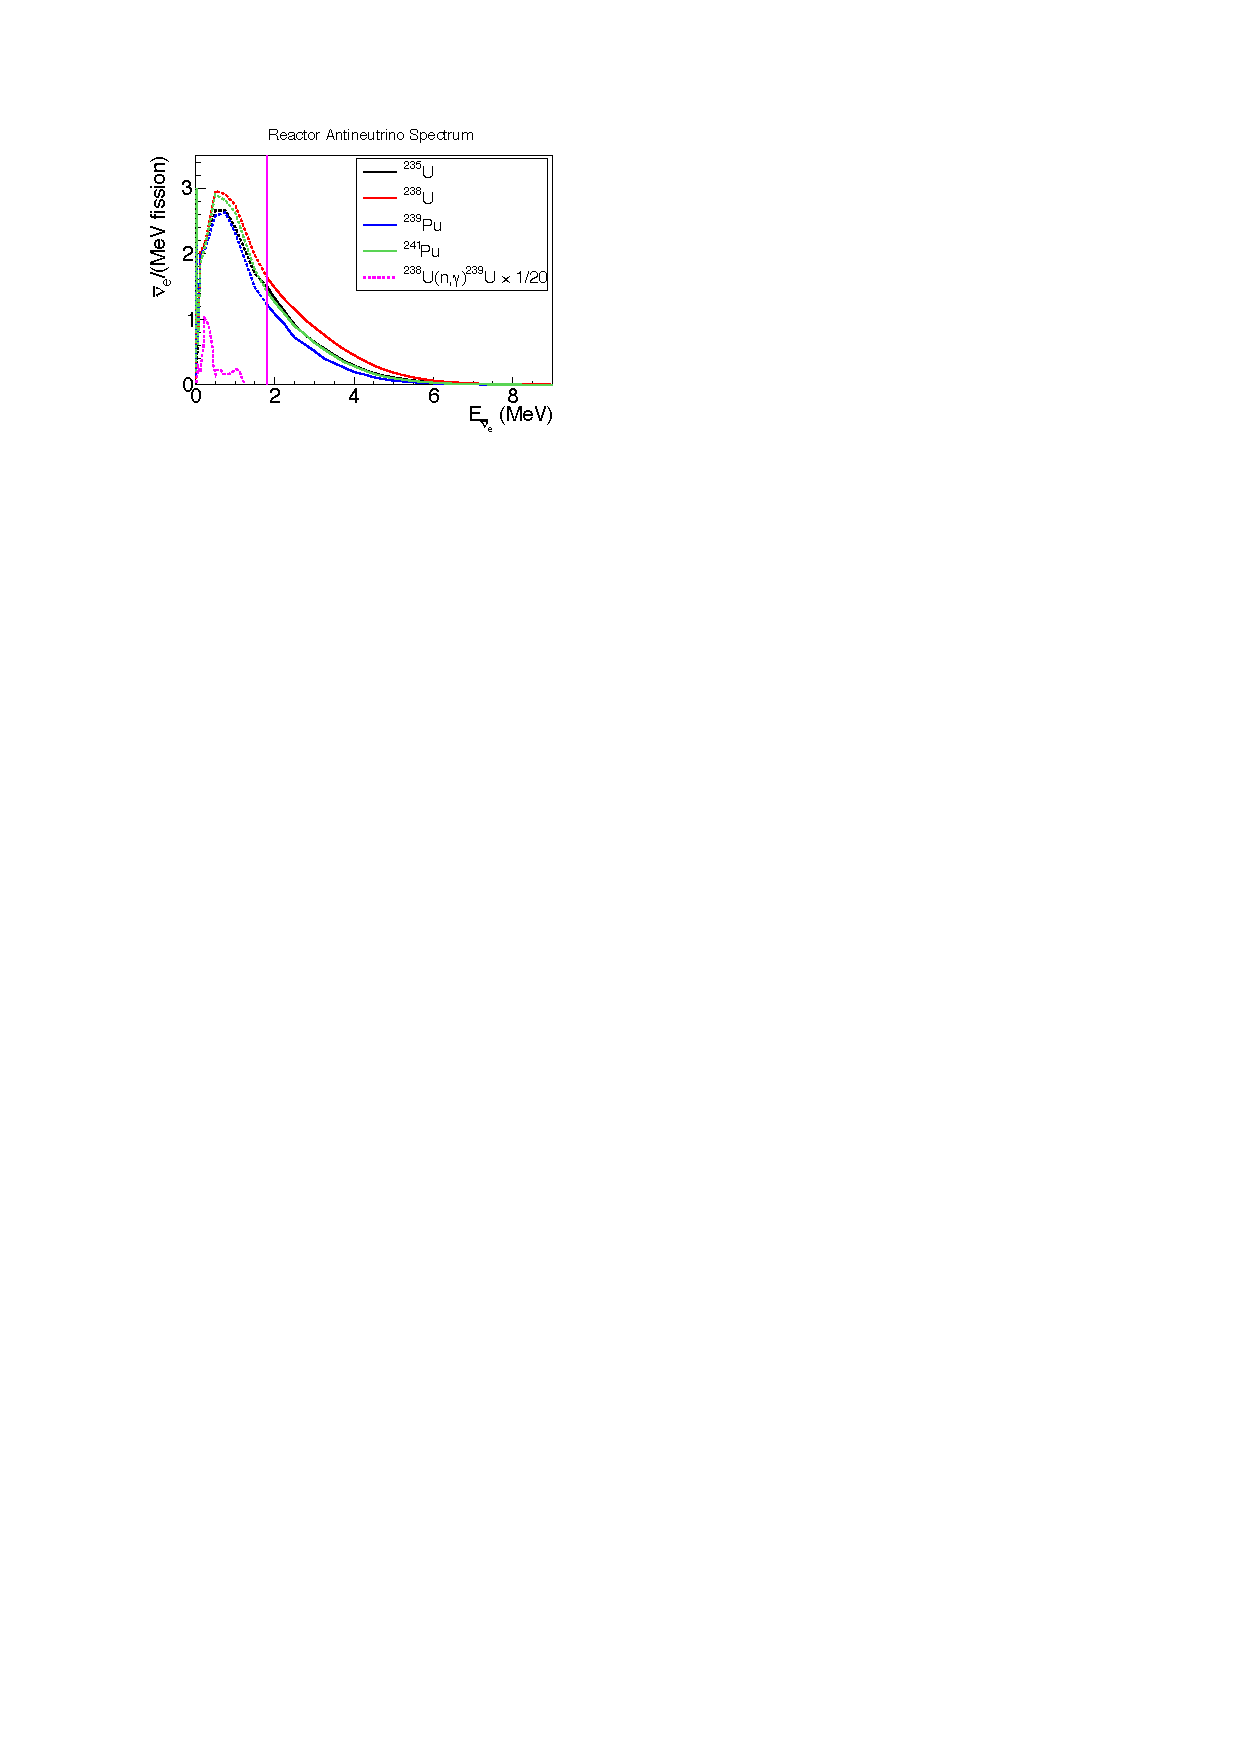
\includegraphics[width=0.5\textwidth]{Figures/RxNeutrinoSpec.pdf}
    \caption[Reactor neutrino spectrum]{An illustration of a commercial reactor neutrino spectrum prediction~\cite{bib:Qian2019}.}
    \end{figure}  

    Reactor neutrino detection experiments rely on the detection of IBD process showed in Equation~\ref{eq1.1}.
    Be cause of the mass difference between neutron and proton, the neutrino energy $E_\nu$ must be above a threshold to trigger the IBD process, as
    \begin{equation}\label{eq2.4}
    E_\nu \ge \frac{(m_n+m+e)^2 - m_p}{2m_p} \simeq 1.806 \textrm{MeV}.
    \end{equation}
    The kinectic energy of the IBD produced neutron $T_n$ is in keV scale.
    Thus, the $e^+$ total energy of IBD can be expressed as
    \begin{equation}\label{eq2.5}
    E_e = E_\nu - (m_n + T_n - m_p) \simeq E_\nu - 1.293 MeV.
    \end{equation}
    In IBD detector, the $e^+$ quickly annihilates with $e^-$ and emits two 0.511~MeV $\gamma$.
    The visible energy of IBD produced $e+$ in an ideal detector is 
    \begin{equation}\label{eq2.6}
    E_{vis} = \simeq E_\nu - 0.782 MeV,
    \end{equation}
    which is a useful experimental conversion for measurement \nuebar energy measurement by measuring the positron energy. 
    The cross-section of the IBD interaction is dependent on the neutrino energy and can be expressed as a function of positron energy
    \begin{equation}\label{eq2.7}
    \sigma_{IBD} \simeq \frac{2\pi^2}{\tau_n m_e^5 f }E_eP_e = 10^{-43}\cdot \frac{E_ep_e}{\textrm{MeV}}\cdot(\frac{\tau_n}{886\textrm{s}})^{-1} \textrm{cm}^2,
    \end{equation} 
    where $\tau$ is neutron life time and $f$ is a phase space integral factor.
    Based on the theoretical neutrino spectrum (Equation~\ref{eq2.2}) and IBD cross-section (Equation~\ref{eq2.7}), an reactor neutrino experiment can expect the measured spectrum and flux as shown in Figure~\ref{fig:2.2}.
    \begin{figure}[h!]
    \centering
    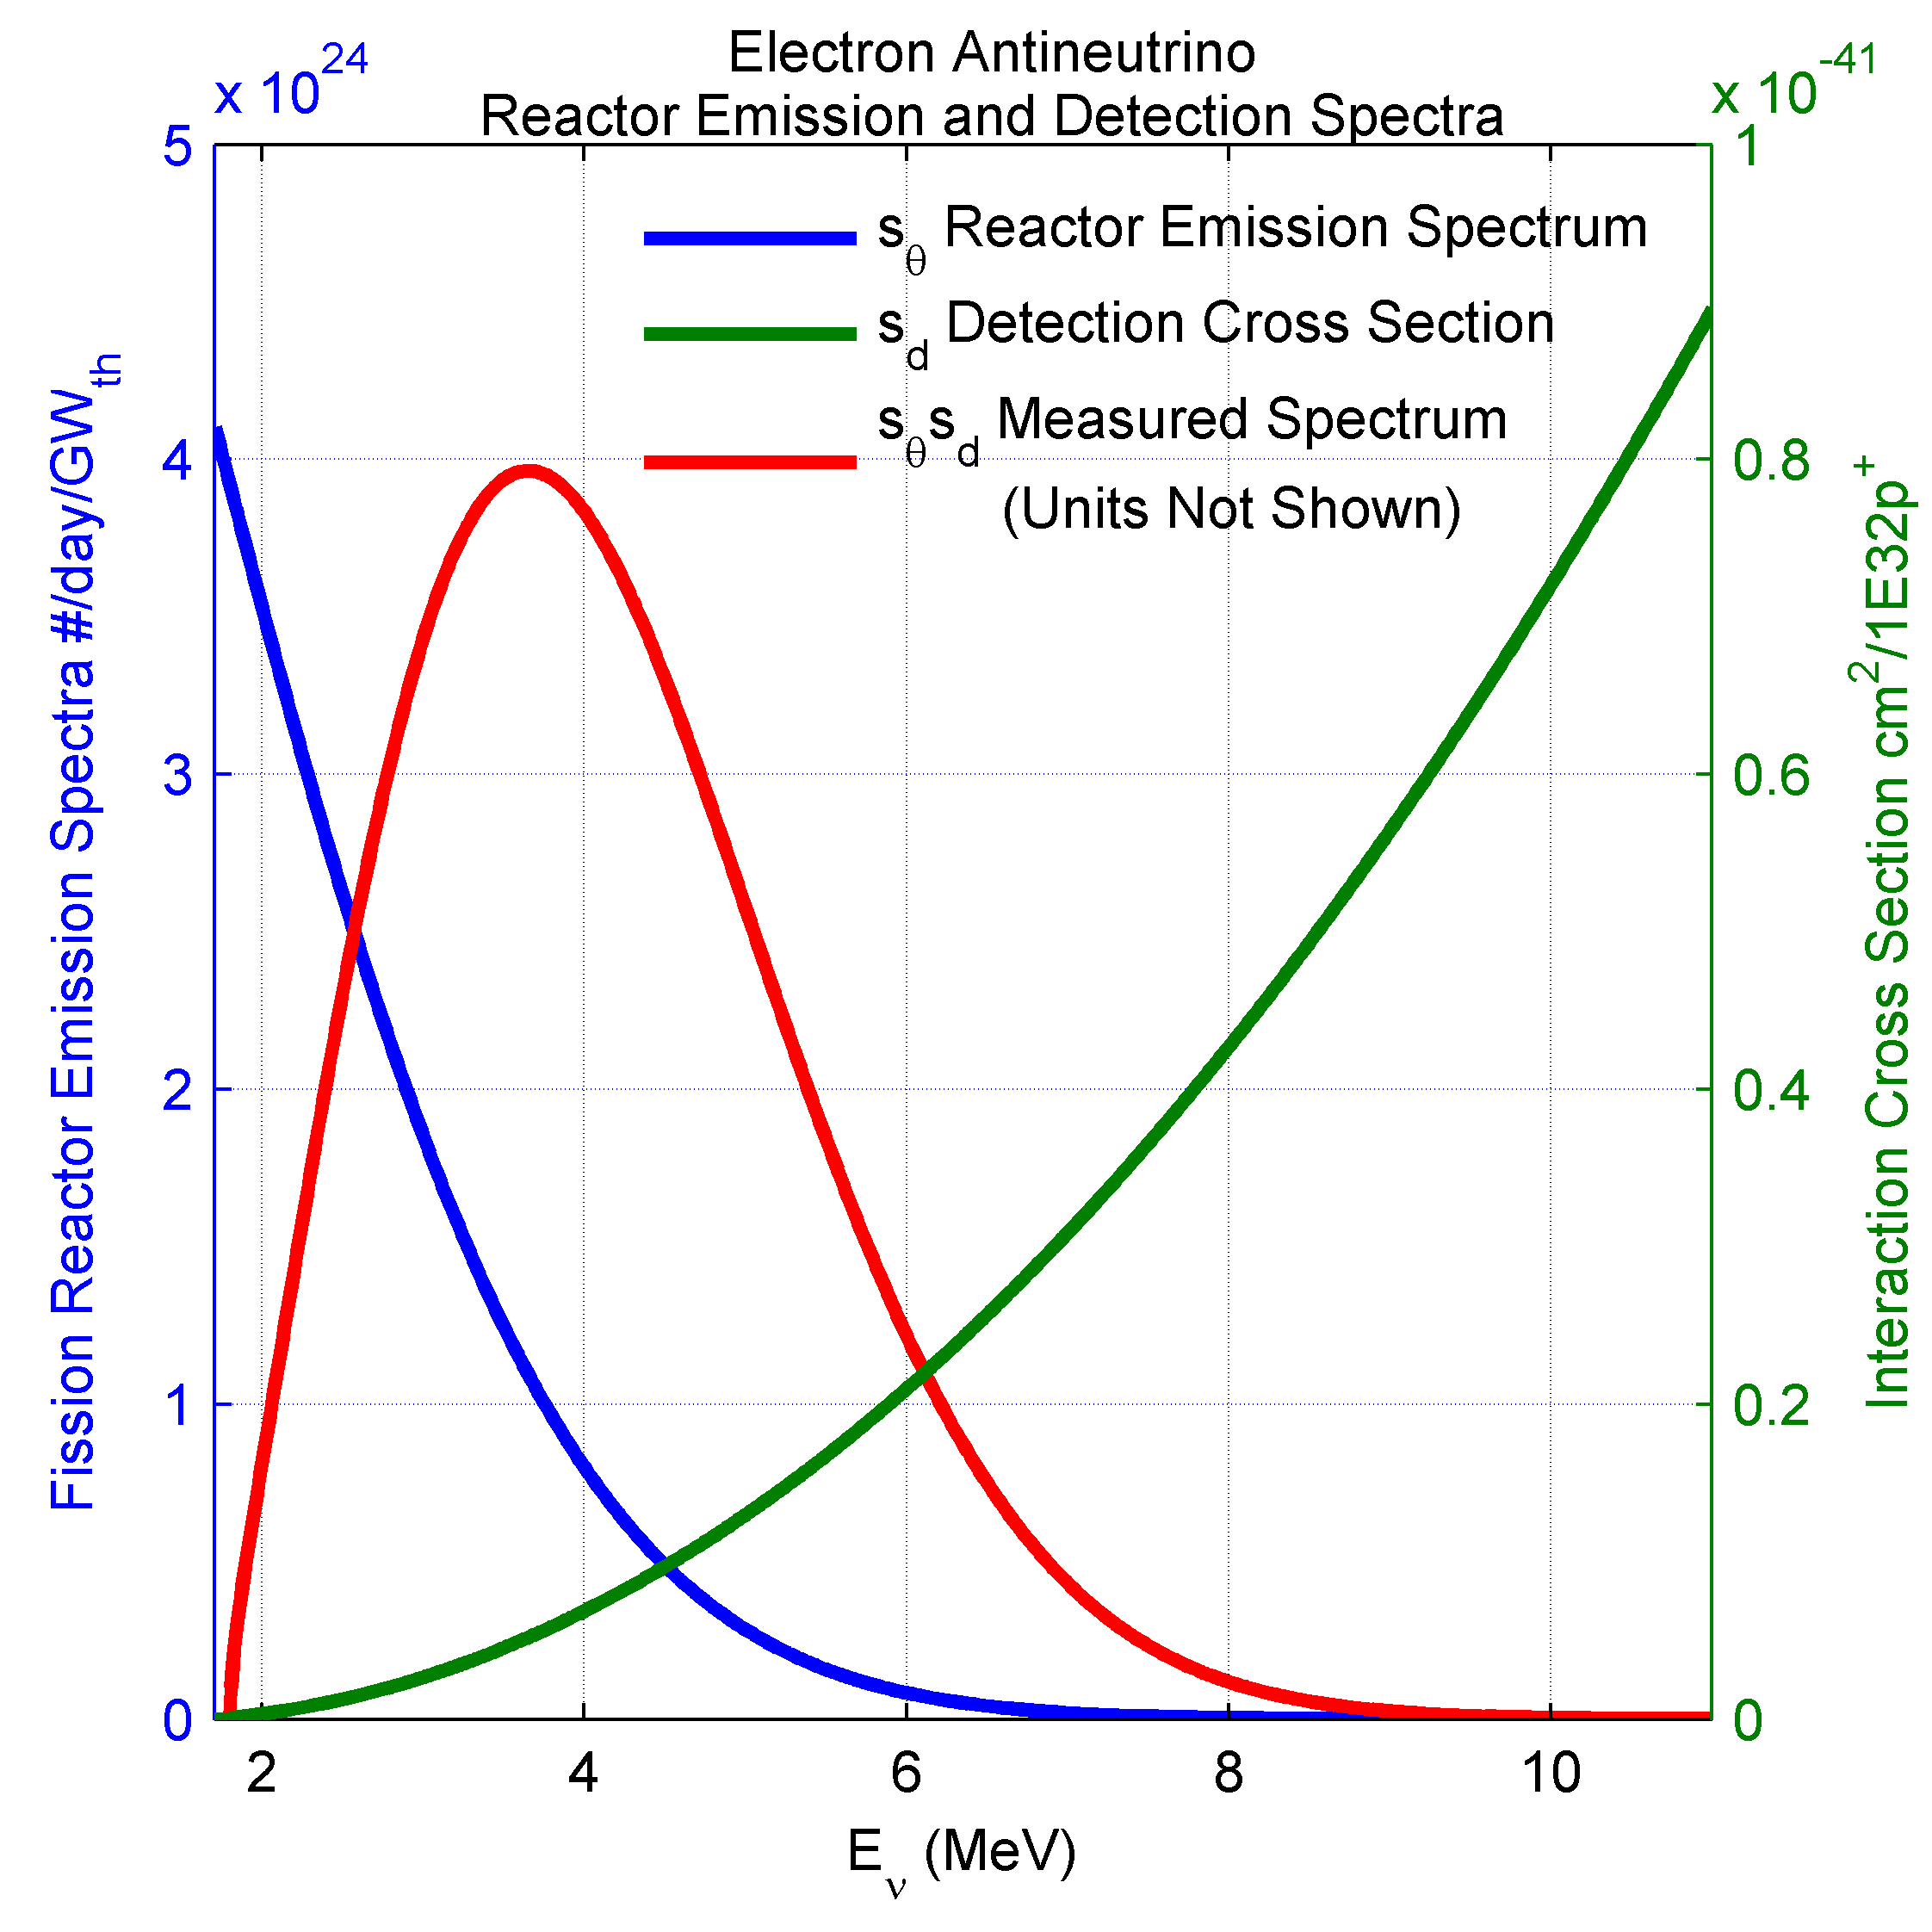
\includegraphics[width=0.6\textwidth]{Figures/twoXsections.png}
    \caption[Detected neutrino spectrum]{An illustration~\cite{bib:Jocher} of the detected neutrino energy spectrum in a reactor experiment. 
    The detected spectrum is the multiplication of the emitted neutrino spectrum and IBD cross-section.}
    \label{fig:2.2}
    \end{figure}      
    
    Reactor neutrino researches have interest of testing the success of nuclear and particle physics by compare experimental measurements of reactor neutrino flux and spectra to the predictions.
    There are two methods to predict the absolute neutrino spectrum of a nuclear reactor:
    \begin{itemize}
        \item \textbf{The \textit{ab initio} method} Neutrino spectrum is calculated by Equation~\ref{eq2.2} and \ref{eq:23}. 
        Where the ratio and the end point energy of each branch is extracted from data in nuclear databases.
        The predicted neutron spectrum is the sum of the calculated $\beta$-spectrum involving theoretical corrections. 
        The neutrino spectrum of $^{238}$U is originally predicted in this way~\cite{bib:vogel}.
        \item \textbf{$\beta$-conversion method} Because the kinetic energy of proton is negligibly small, the total $\beta$-decay end point energy $E_0 \simeq E_\nu + E_e$.
        The neutrino spectrum can be deduced from the experimental measurement of $\beta$ energy from fission reactor. 
        In 1980s, the $^{235}$U, $^{239}$Pu, and $^{241}$Pu neutrino spectra was converted from the spectrum measurements of $\beta$ from the Institut Laue-Langevin (ILL) reactor~\cite{bib:ILL1982,bib:ILL1985,bib:ILL1989}.
        The conversion was made by fitting the measured $\beta$ spectrum with sum of tens of hypothetical $\beta$-decay branches, then converting the spectrum of each $\beta$ branch to neutrino spectrum with respect to the best-fit branch ratio.
    \end{itemize}
    The detailed theoretical approaches are described in Section 3 of this chapter. 
    
    Successful neutrino flux and spectrum prediction and measurement made it possible for reactor neutrino experiments to test nuclear model of fission reactors.

\Section{Historical Context of Reactor Neutrino Experiments}

    After neutrino's discovery through the detection by the Savannah reactor neutrino experiment~\cite{bib:CowanReines},
    a hint of $\nuebar$ oscillation was discovered by Reines \textit{et al} in 1980~\cite{bib:reines1980}.
    Their experiment found in unexpected ratio charged current and neutral current interaction with $2\sigma-3\sigma$, which suggests antineutrino oscillation.
    More reactor experiments were built to test \nuebar oscillation covering a big variety of baseline by comparing neutrino flux to the theoretical predictions or between different baselines, included in Table~\ref{tab:history}.
    These experiments attempted to observe neutrino oscillation through \nuebar disappearance.
    The commonly used methods are to compare the observed neutrino flux to the expected flux, or to compare the relative flux/spectrum difference at different baselines.
    \begin{table}[!htbp]
    \centering
    \caption[Historical reactor oscillation experiments]{The historical reactor experiments searching for \nuebar oscillation in baseline from $\sim$10~m to $\sim$100~km.}
    \begin{tabular}{lllll}
    \hline
    Experiment  & Baseline   & Absolute Flux  & Relative Flux    & Reference   \\ 
    \hline
    ILL     & 8.76~m  & $0.955\pm 0.115$  &  & \cite{bib:kwon1981}  \\
    \hline
        & 37.9~m   & $1.018\pm 0.06$  &   &   \\
    G\"osgen  & 45.9~m  & $1.045\pm 0.06$  &   & \cite{bib:gosgen}  \\
        & 64.7~m    & $0.975\pm 0.06$  &   &   \\
    \hline
    Rovno     & 18.3~m to 25.3~m     & $0.964\pm 0.068$  &   & \cite{bib:Afonin1987}  \\
    \hline
    Krasnoyarsk     &  57~m to 231~m    & $0.99\pm 0.05$  & $0.86\pm 0.15$  &  \cite{bib:Vidyakin1994} \\
    \hline
        & 14~m & $0.988\pm 0.05$  &   &   \\
    Bugey   & 40~m  & $0.994\pm 0.05$  &   &  \cite{bib:Bugey} \\
        & 95~m  & $0.913\pm 0.13$  &   &   \\
    \hline
    Savannah River  &  18~m & $0.987\pm 0.038$ &    & \cite{bib:Greenwood1996} \\
        &4~m    & $1.055\pm 0.038$  &   &   \\
    \hline
    CHOOZ   & 1~km     & $1.01\pm 0.04$   &   & \cite{bib:chooz98, bib:Chooz99, bib:chooz03}  \\
    \hline
    Palo Verde   &  750~m to 890~m & $1.04\pm 0.09$ &   &  \cite{bib:palo01, bib:palo1999, bib:palo2000} \\
    \hline
    KamLAND & 80~km to 800~km  &  $0.658\pm 0.06$ &   & \cite{bib:KamLAND03, bib:kamland04}  \\
    \hline
    \end{tabular}
    \label{tab:history}
    \end{table}
 
    The experiments listed in Table~2.1 covered different $(\Delta m^2, \sin^2\theta)$ parameter space of neutrino oscillation.
    CHOOZ and Palo Verde experiments narrowed the allowed range of the parameter space by $\sin^2 2\theta_{13} \le 0.18$ for $|\Delta m^2_{13}|\ge 2\times 10^{-3}$ eV$^2$, suggesting the $\nu_\mu \rightarrow \nu_e$ oscillation is small in atmosphere neutrino anomaly.
    
    In 2002, KamLAND experiment~\cite{bib:KamLAND03, bib:kamland04} confirmed the reactor \nuebar oscillation by spectrum measurement of \nuebar from mainly 53 reactors around Japan (also 5\% in South Korea and 1\% global), with 180~km average baseline.
    KamLAND experiment utilized spherical detector with filled about 3000~ton LS deployed in the Kamioka mine in Japan. 
    The IBD positron and neutron signals are collected by 1879 inward facing PMTs on the surface of the detector. 
    Similar to the Cowan-Reines experiment~\cite{bib:CowanReines}, KamLAND used positron-neutron time coincidence to tag the IBD interaction candidates, the prompt positron signal is followed by a delayed $\gamma$ signal from $n$-Gd capture in the detector.
    With 162 ton$\cdot$yr \nuebar rate, KamLAND experiment observed neutrino oscillation in the very long baseline by comparing detected neutrino flux to neutrino flux predicted by the ILL+Vogel model~\cite{bib:ILL1982, bib:ILL1985, bib:ILL1989, bib:vogel} showed in Figure~\ref{fig:kamFlux}.
    KamLAND also observed the oscillation behavior dependent on $L/E$ ratio showed~\ref{fig:kamLE}.
    
    \begin{figure}[h!]
    \centering
    \subfigure[]{\label{fig:kamFlux}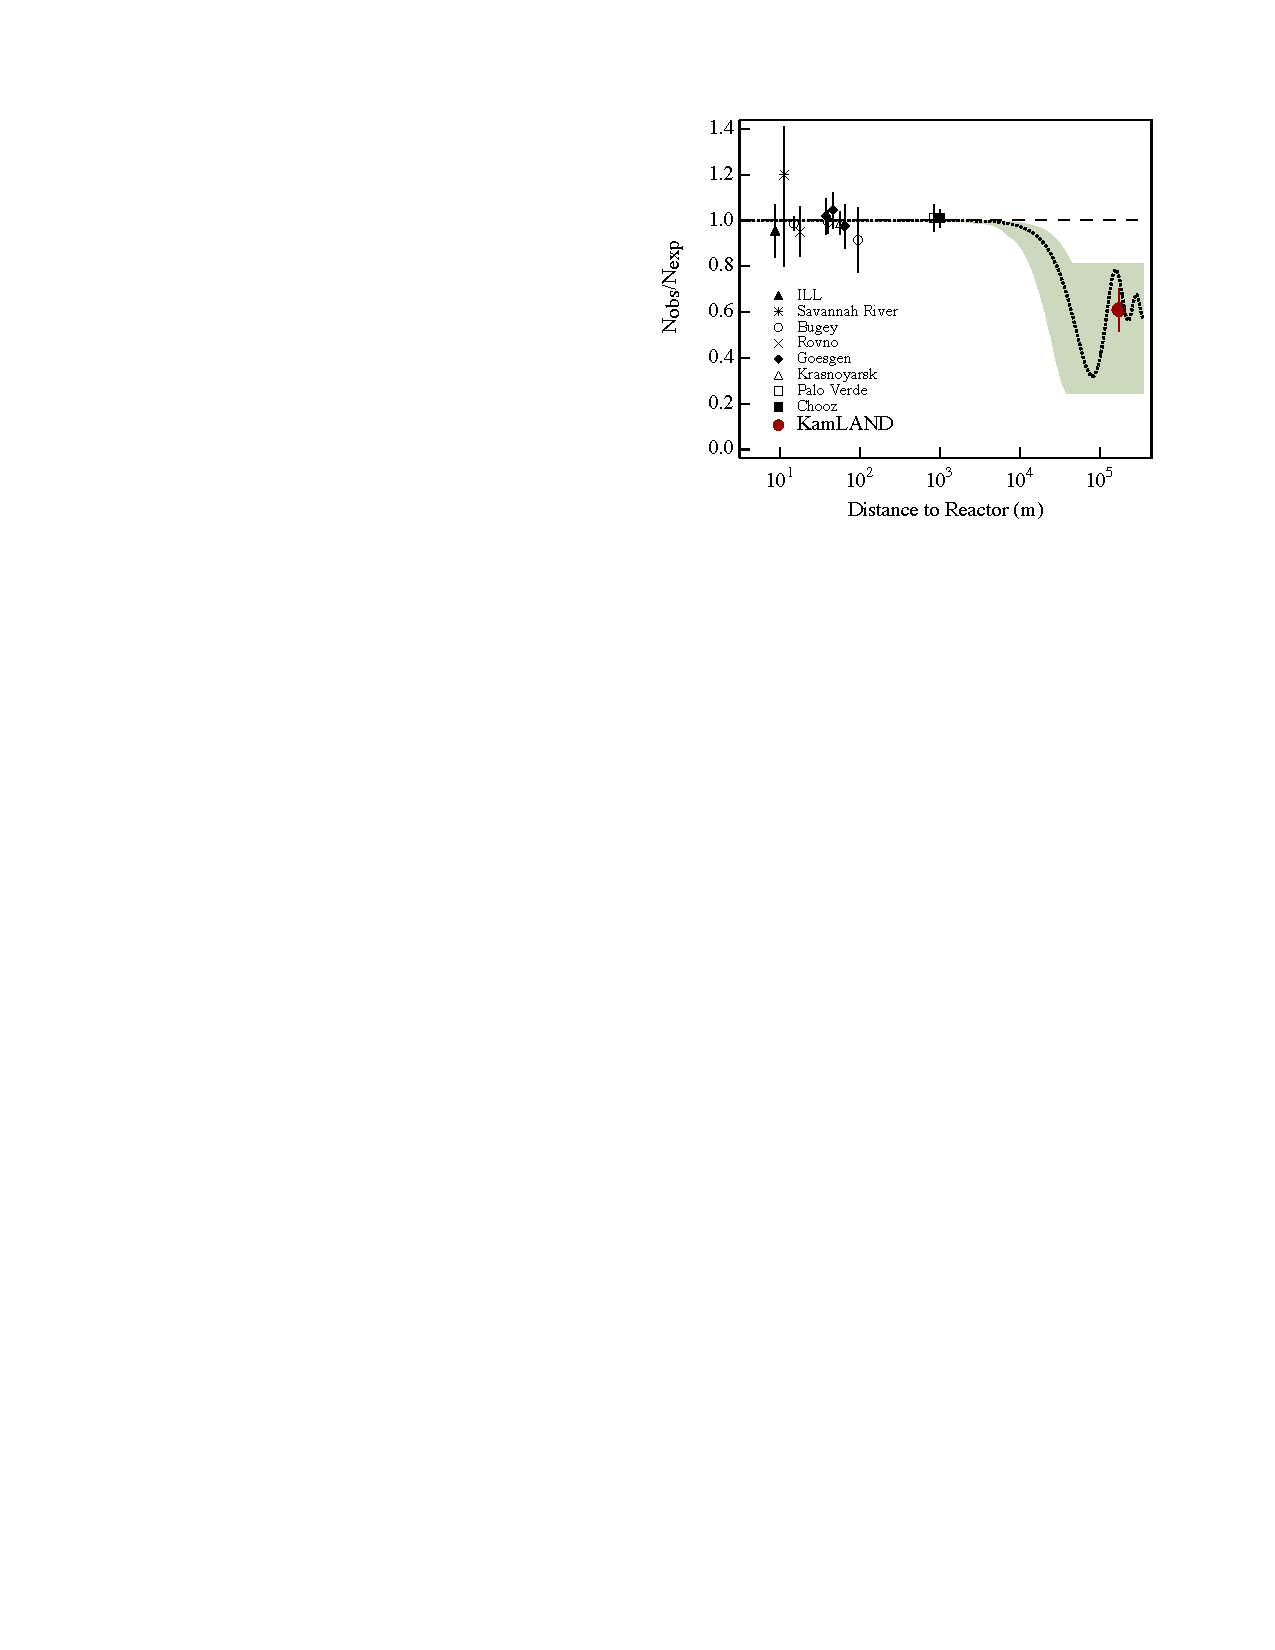
\includegraphics[width=60mm]{Figures/KamLANDFlux.pdf}}
    \subfigure[]{\label{fig:kamLE}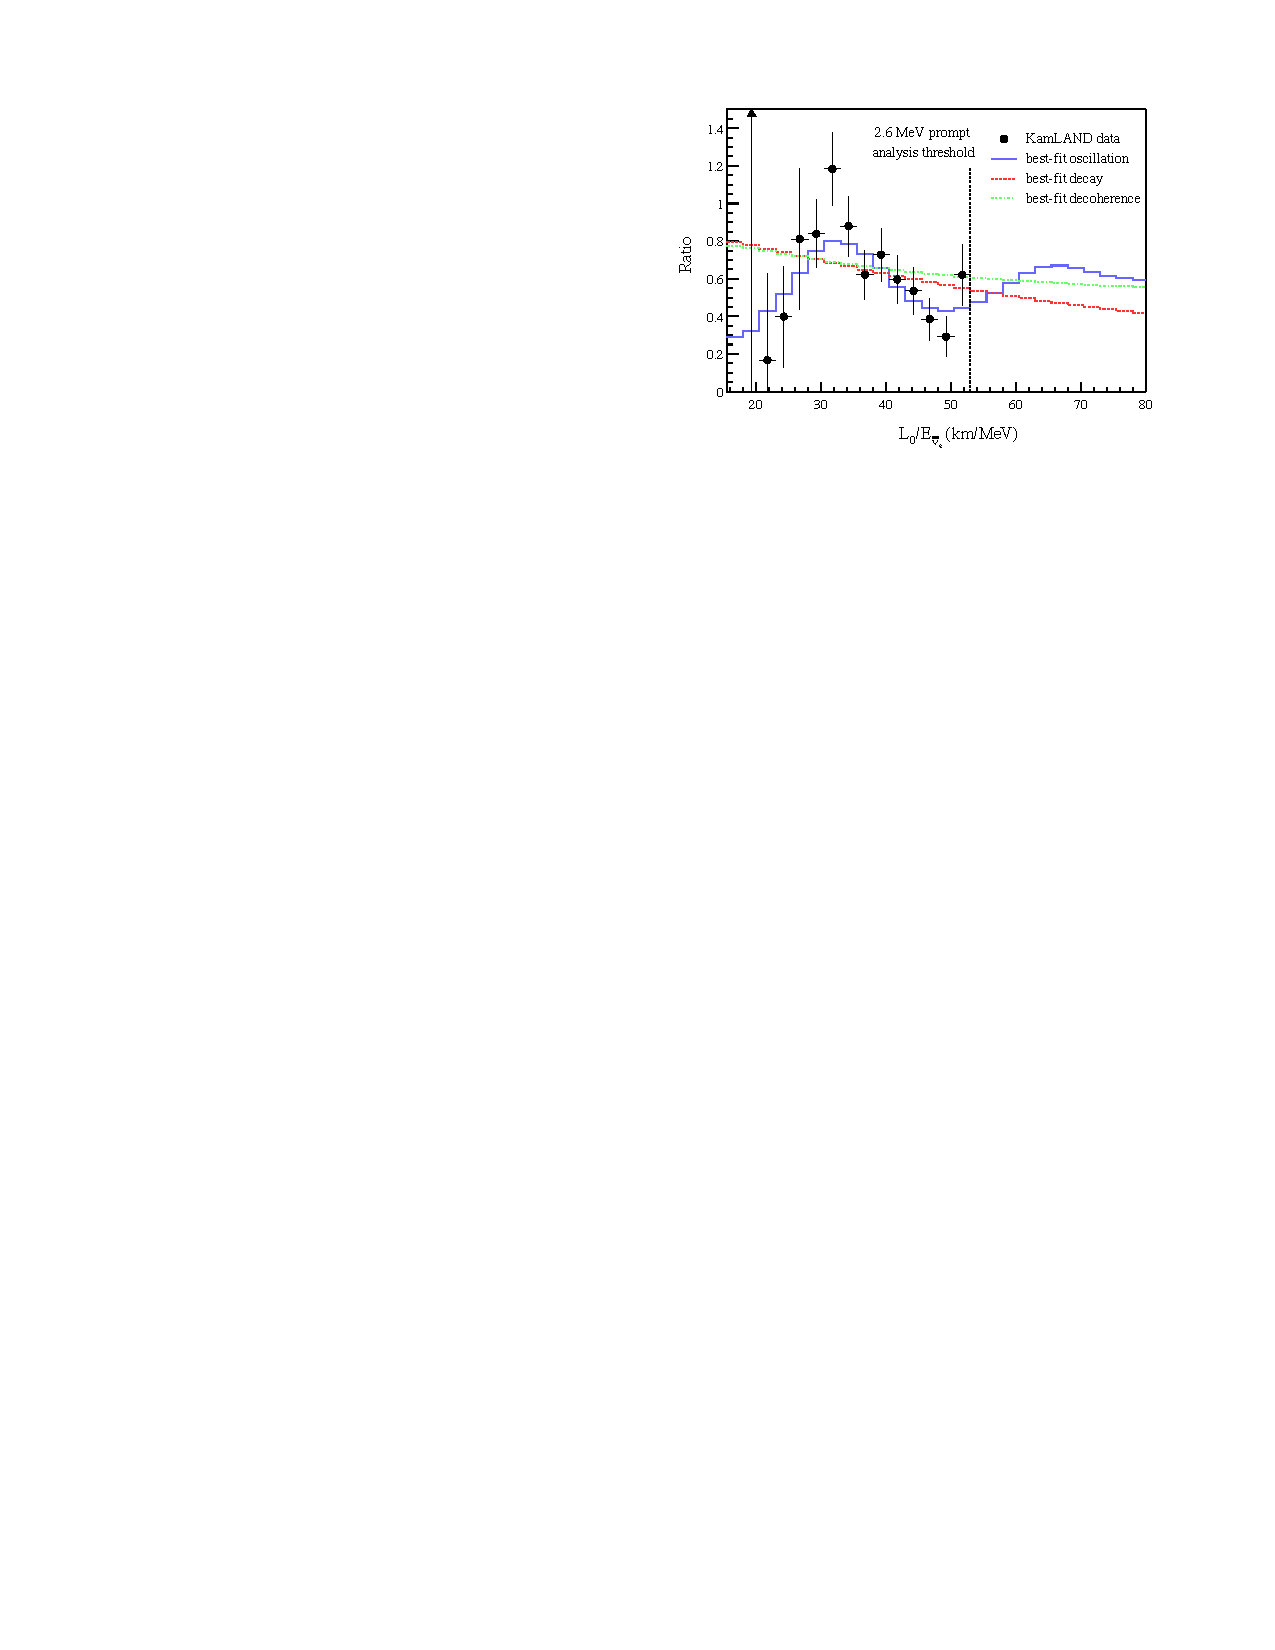
\includegraphics[width=60mm]{Figures/KamLANDLE.pdf}}
    \caption[Confirmation of Reactor Neutrino Oscillation by KamLAND]{The observation of reactor neutrino oscillation by KamLAND.
    (a) The ratio of the KamLAND observed neutrino flux to ILL+Vogel prediction.
    (b) The ratio of KamLAND measured $L_0/E$ spectrum to no oscillation prediction with average baseline $L_0 = 180$~km, indicating oscillation behavior with respect to $L_0/E$ of \nuebar.
    This result also disfavored neutron decay and decoherence model made based on atmosphere neutrino experiment.}
    \label{fig:Kamland}
    \end{figure}
    
    Another milestone in the reactor neutrino experiments is the precise measurement of the $\theta_{13}$ mixing angle. 
    Historically, the medium baseline experiments, CHOOZ~\cite{bib:chooz03}, Parlo Verde~\cite{bib:palo2000}, RENO~\cite{bib:RENO}, Daya Bay~\cite{bib:DYBosc} and Double CHOOZ~\cite{bib:DBChooz} experiments attempted to measure $\theta_{13}$ by observing the $\nuebar\rightarrow\nuebar$ disappearance in baselines varying from several hundred meter to 1~km from commercial reactors.
    Following CHOOZ and Parlo Verde's measurement of the $\sin^22\theta_{13}$ upper bound, RENO, Daya Bay and Double CHOOZ independently reported the measurement of non-zero $\theta_{13}$ mixing angle.
    The three $\theta_{13}$ experiments all utilized Gd loaded LS detectors deployed at different baselines from groups reactors.
    By comparing the \nuebar flux between near and far detectors, these experiments measured the $\nuebar\rightarrow\nuebar$ disappearance probability independently from nuclear model of the reactors.
    The result of the measurements is shown in Table~\ref{tab:1.1}.
    The commercial reactors utilized in these experiments are contains various effective fission fractions that evolve with time.
    \begin{table}[h]
    \centering
    \caption[$\theta_{13}$ reactor experiments]{The medium baseline reactor neutrino experiments that measured $\theta_{13}$ mixing angle.
}
    \begin{tabular}{ccc}
    \hline
    \hline
    Experiment  & Baseline   & Average Fission Fraction   \\ 
    \hline
    Daya Bay     & 560~m to 1640~m  & 5.71\% $^{235}$U, 29.9\% $^{239}$Pu, 7.6\% $^{238}$U, 5.4\% $^{241}$Pu \\
    RENO     & 294~m to 1383~m & 5.73\% $^{235}$U, 29.9\% $^{239}$Pu, 7.3\% $^{238}$U, 5.5\% $^{241}$Pu \\
    Double CHOOZ    & 1050~m & 48.8\% $^{235}$U, 35.9\% $^{239}$Pu, 8.7\% $^{238}$U, 6.7\% $^{241}$Pu \\
    \hline
    \end{tabular}
    \label{tab:theta13}
    \end{table}

\Section{Reactor Antineutrino Anomaly}
\label{c2s3}
        
    In addition to the oscillation measurement, the $\theta_{13}$ experiments also measured absolute neutrino flux and spectrum of commercial reactors. 
    To provide precise models for these measurements, predictions of reactor neutrino flux and spectrum is revisited with both the \textit{ab initio} method and the $\beta$ conversion method.
    
    The Mueller model~\cite{bib:mueller} read the ENSDF and JENDL nuclear databases to sum the \nuebar spectrum from the $\beta$ branches.
    This method also used the branching fraction of from the databases to fit the ILL measurement in 1980s and calculated the \nuebar spectra of $^{235}$U, $^{238}$U, $^{239}$Pu, and $^{241}$Pu.
    The Huber model~\cite{bib:huber} utilized the $\beta$ spectra of $^{235}$U, $^{239}$Pu, and $^{241}$Pu measured from the ILL reactor and applied the conversion method with higher order theoretical corrections to the $\beta$ spectra of the virtual decay branches.
    The theoretical corrections include the effect of electron-nucleus interaction, photon radiation, and weak magnetism correction. 
    With different approaches of theoretical distribution, Mueller model of expected neutrino flux found 2.5\% more than the ILL+Vogel model, and Huber model found 3\% increase in neutrino flux prediction.
    However, the absolute flux measurements of the historical reactor experiments within 1~km baseline showed inconsistent reactor neutrino flux with either of the prediction, as shown in Figure~\ref{fig:DYBFlux}.
    \begin{figure}[h!]
    \centering
    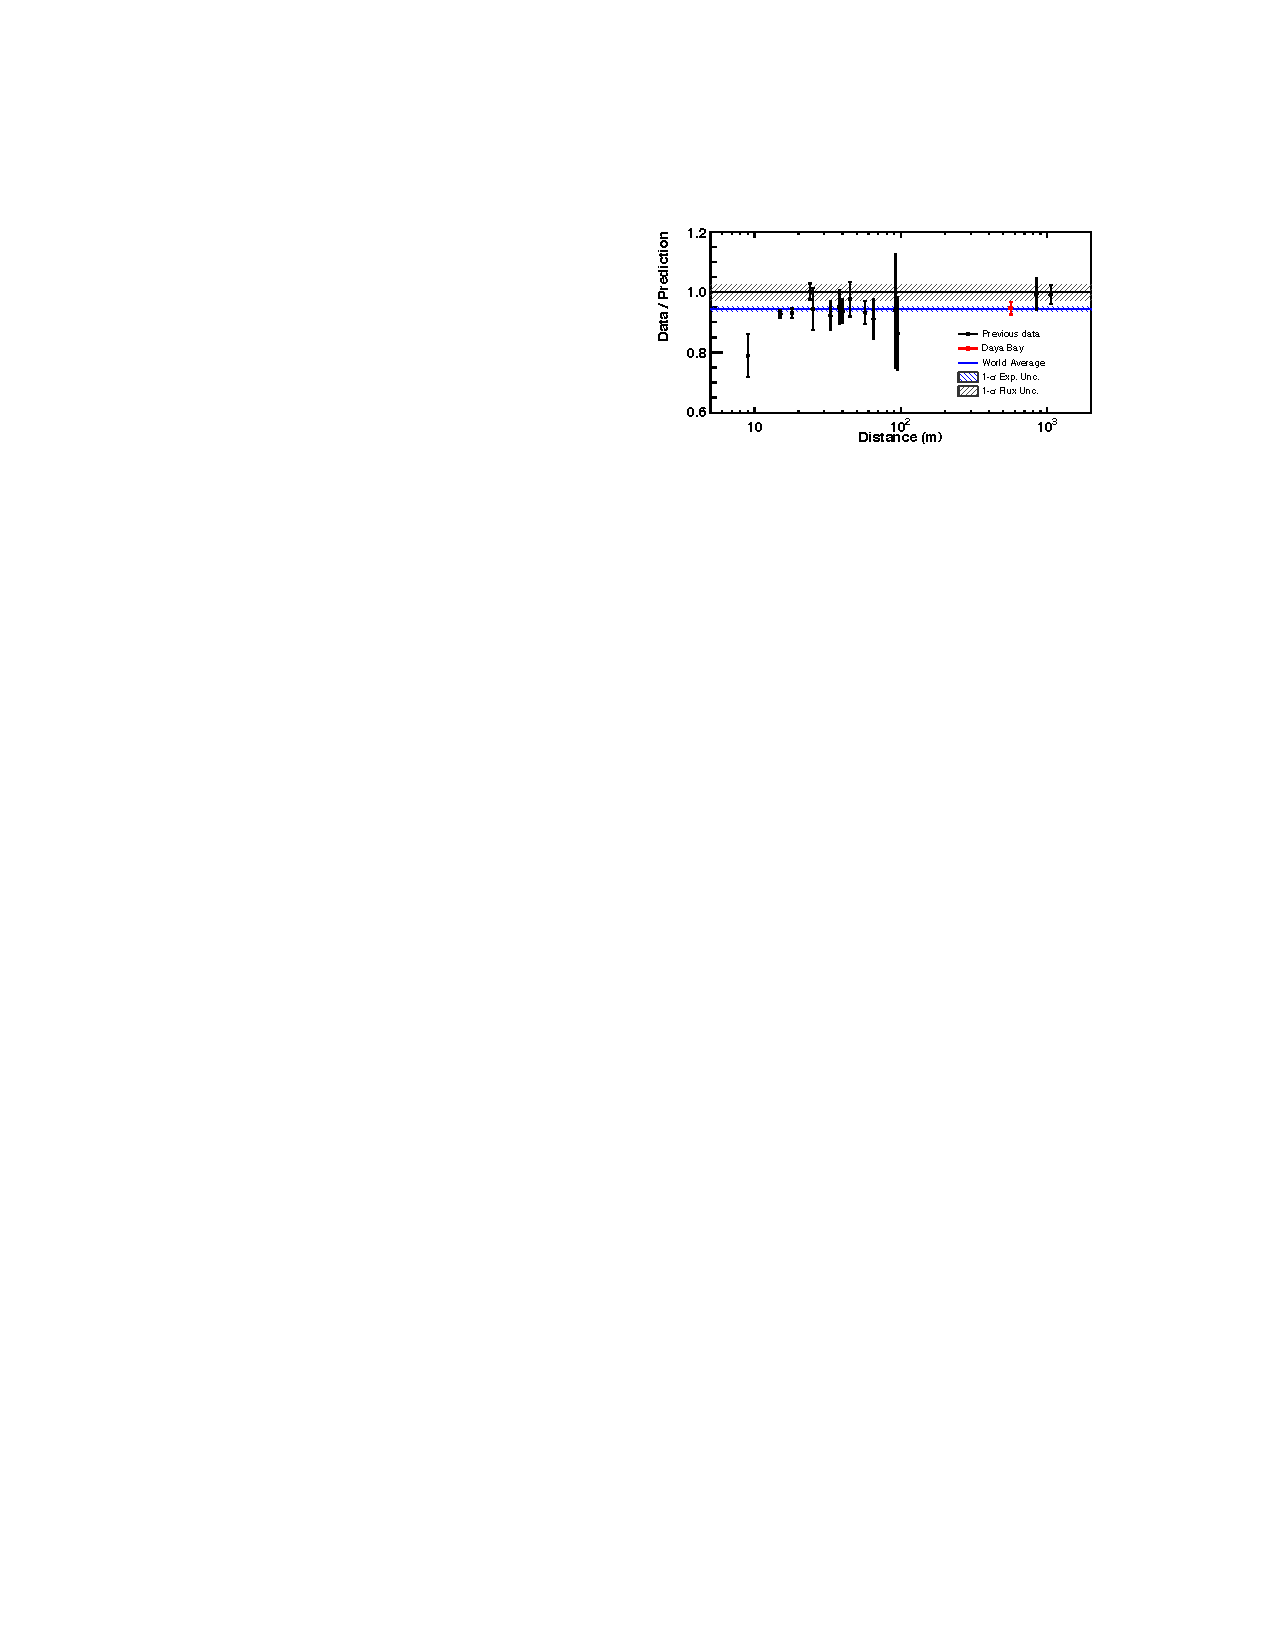
\includegraphics[width=0.6\textwidth]{Figures/DYBGlobalFlux.pdf}
    \caption[Daya Bay Absolute Reactor Neutrino Flux]{Historical reactor neutrino flux measurements \cite{bib:DYB2015}.
    The global average is 5\% to 6\% deficit from Huber+Mueller predicted flux.}
    \label{fig:DYBFlux}
    \end{figure}
    
    The neutrino flux deviation is referred as the Reactor Antineutrino Anomaly (RAA)~\cite{bib:RAA}.
    This anomaly suggests a systematic bias present in the theoretical aggregation method and/or the virtual branching approach in the conversion from the ILL measured $\beta$ spectrum.
    This disagreement of neutrino flux in the medium baselines can also be explained by a possible oscillation between \nuebar and a light sterile neutrino.
    A 3+1 model of left hand neutrino mixing with sterile neutrino with $\Delta m^2$ in $\sim$1~eV$^2$ scale is developed based on the disappearance rate shown in the flux deficit.
    The RAA best fit 3+1 neutrino oscillation parameters are shown in Figure~\ref{fig:RAA}.
\begin{figure}[h!]
    \centering
    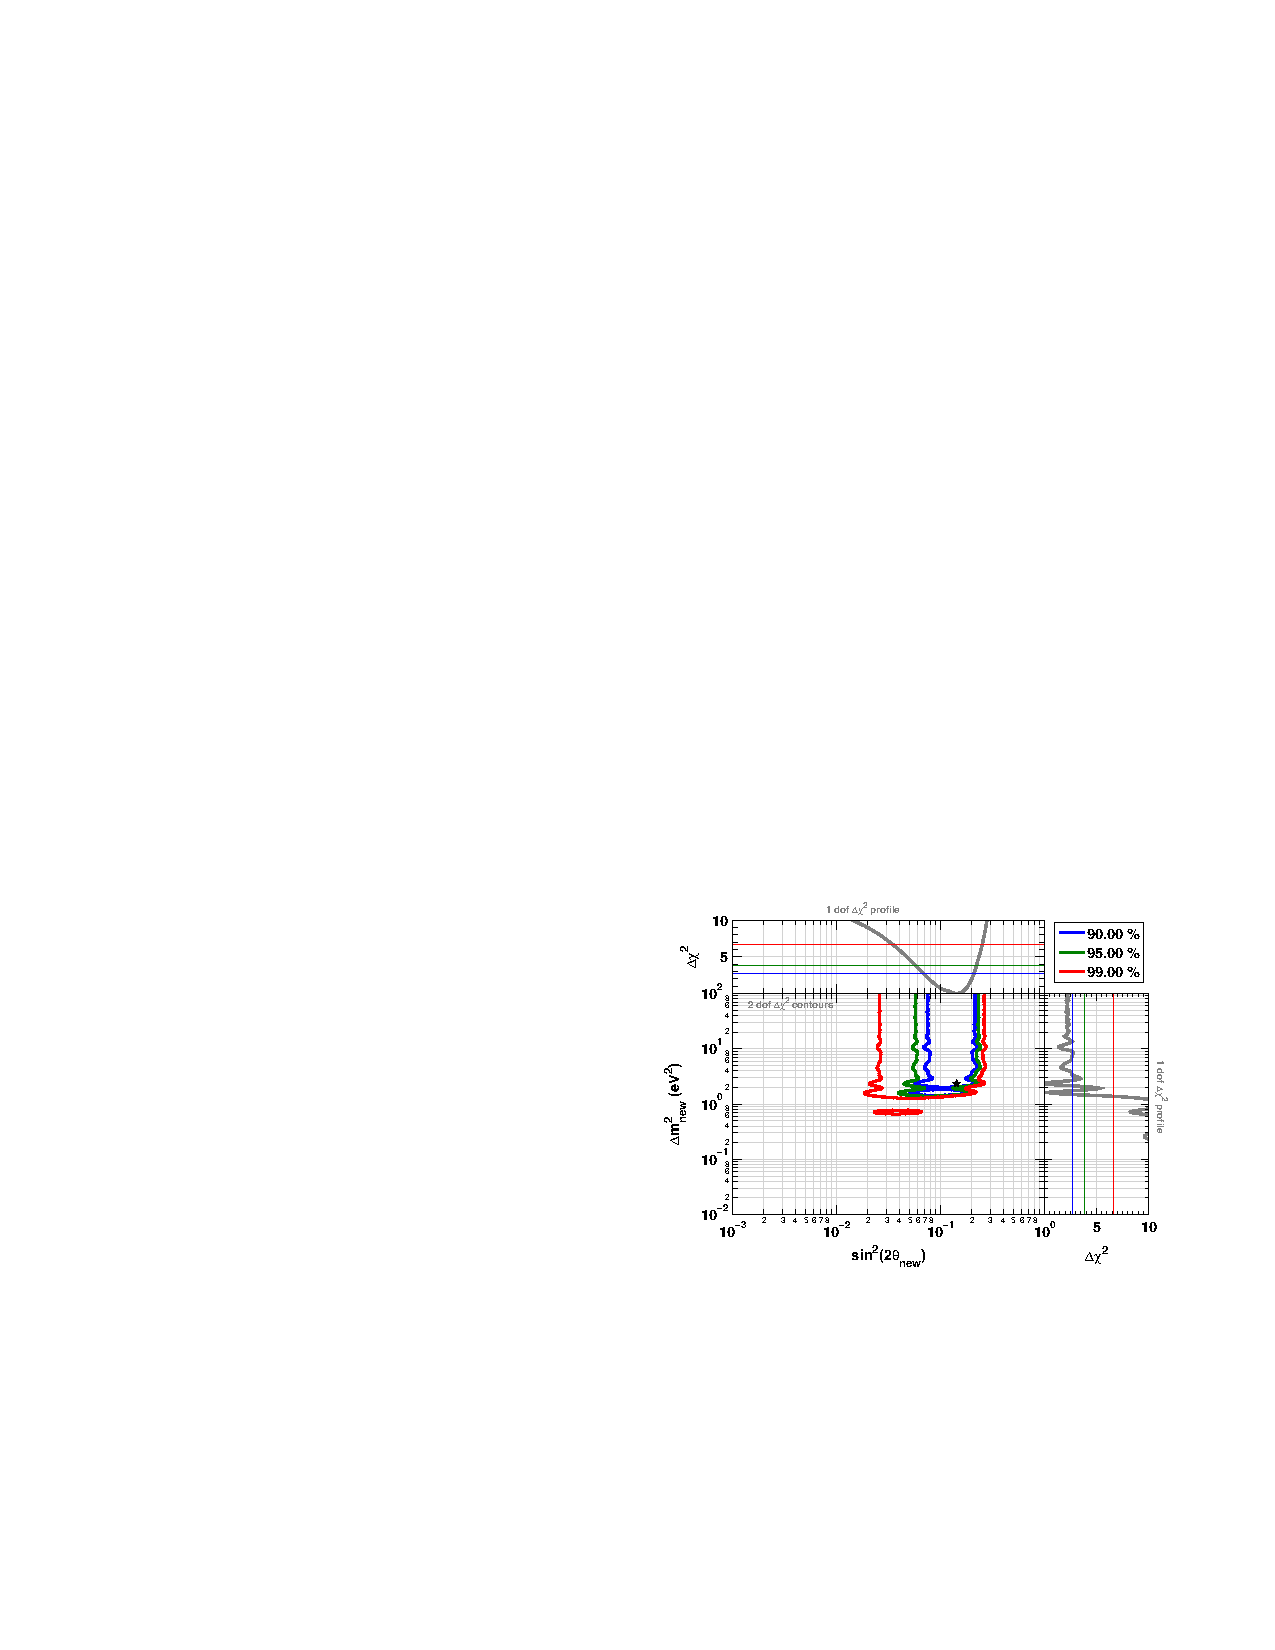
\includegraphics[width=0.6\textwidth]{Figures/RAA3plus1.pdf}
    \caption[The allowed region for the parameters of sterile oscillation]{The allowed region for the parameters of the sterile neutrino oscillation as a result of the flux deficit observed in RAA~\cite{bib:RAA}. The best fit point suggests a $\sin_{14}^22\theta = 0.14\pm0.08$ and $|\Delta m^2| > 1.5$~eV$^2$ (95\% C.L.) of a 3+1 left hand neutrino and sterile neutrino mixing.}
    \label{fig:RAA}
\end{figure}

    In dependent of the flux deviation, the medium baseline experiments, Daya Bay~\cite{bib:DYBSpectrum}, Double CHOOZ~\cite{bib:DBChooz} and RENO~\cite{bib:RENO}, also measured reactor neutrino spectrum disagreeing to the Huber and Mueller models, as shown in Figure~\ref{fig:DYBSpectrum}.
    An 8\% to 10\% excess is observed in the 4~MeV to 6~MeV region of IBD positron energy, equivalent to 5~MeV to 7~MeV reactor neutrino energy.
    With high statistical significance, the spectral deficit also hints errors in the nuclear database used to calculate the expected spectral shape.
    Additionally, the isotopic contribution to the flux and spectrum anomaly is unclear due to the mixture and evolution of the fission isotopes in Low Enrichment Uranium (LEU) reactors utilized by these experiments.
 \begin{figure}[h!]
    \centering
    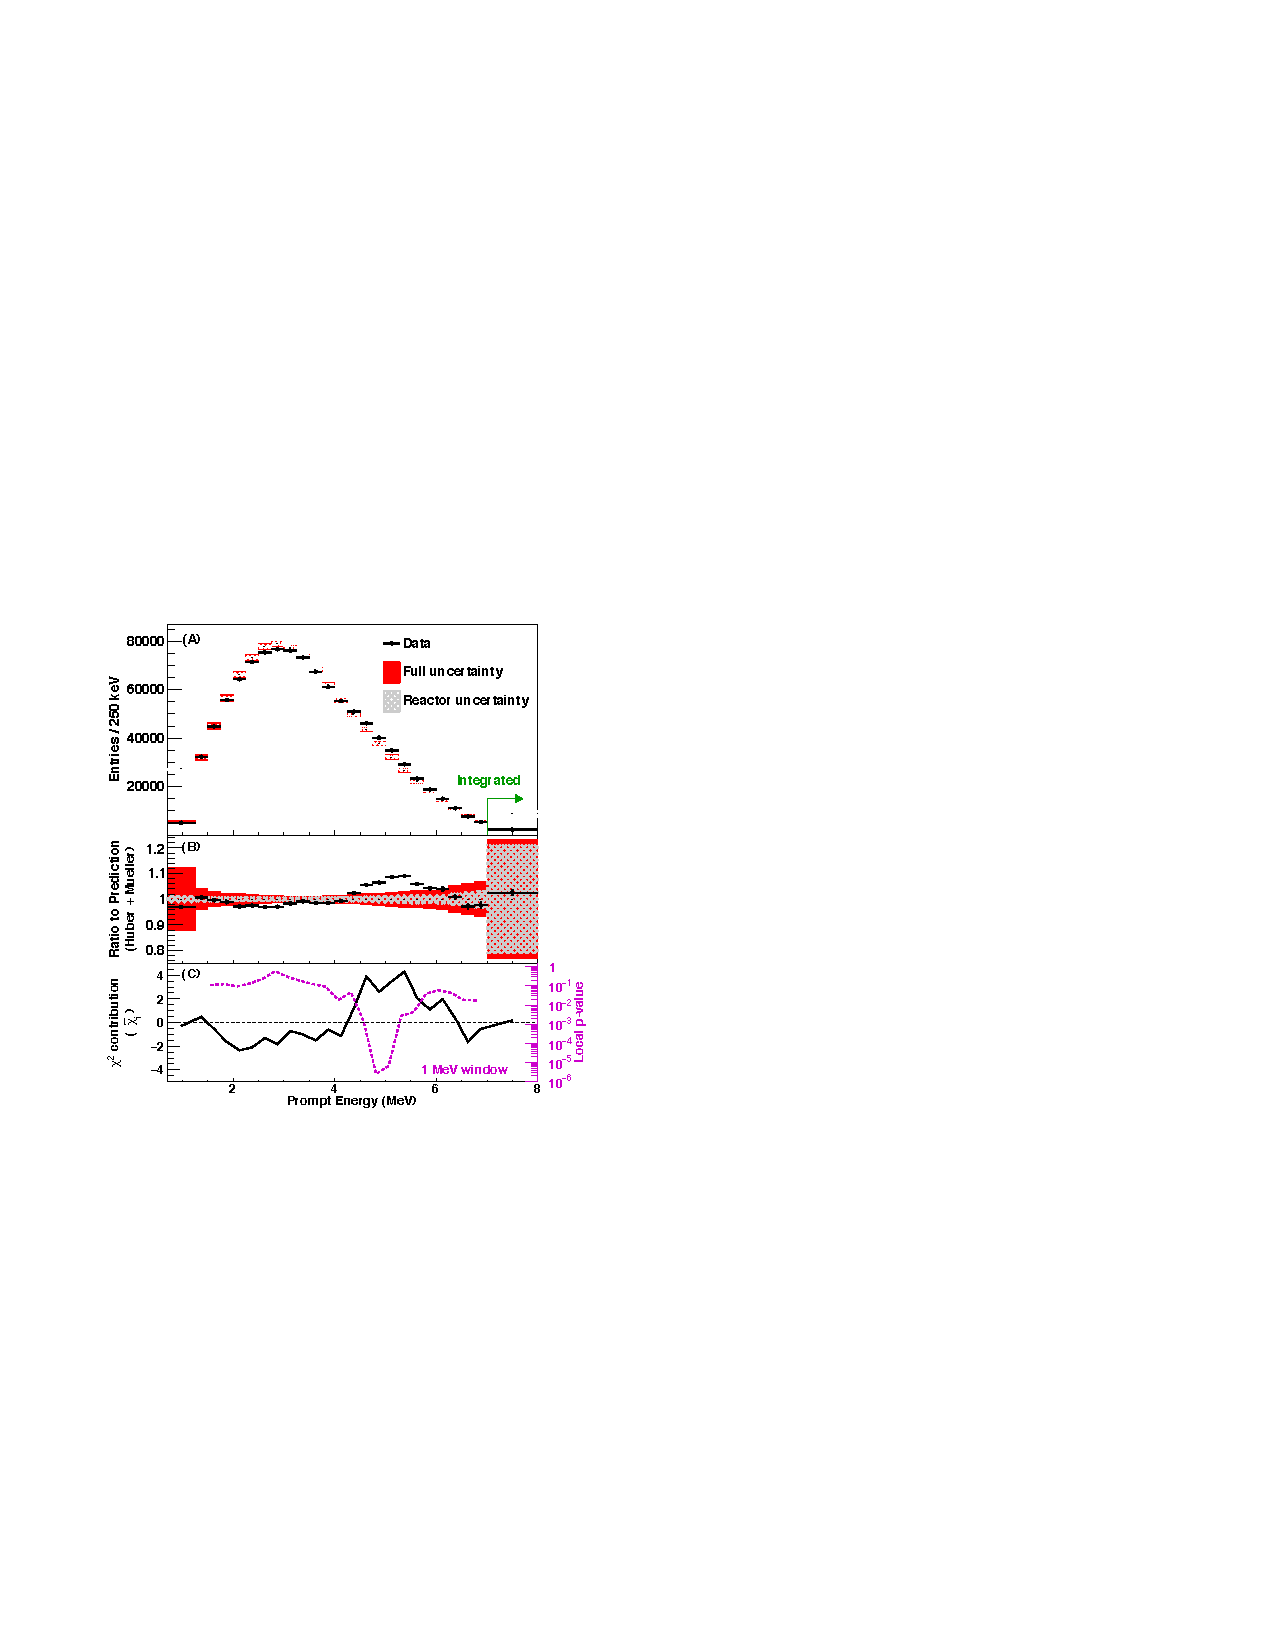
\includegraphics[width=0.6\textwidth]{Figures/DYBSpectrum.pdf}
    \caption[Daya Bay IBD positron energy spectrum]{The IBD positron energy spectrum measured by Daya Bay experiment.
    The spectrum is the sum of IBD positron spectrum from four fission isotopes, which indicate an excess at 4~MeV to 6~MeV compared to the Huber+Mueller model with 2.9~$\sigma$ discrepancy.}
    \label{fig:DYBSpectrum}
    
\end{figure} 
    
\Section{Resolution to the RAA}

    Further studies, including introducing forbidden transition in fission branches~\cite{bib:hayes} and \textit{ab initio} spectrum prediction with different nuclear databases~\cite{bib:dwyer}.
    These studies suggested larger systematic uncertainty of branching in Huber+Mueller model because of the lack of forbidden branching knowledge and errors in nuclear databases.
    Phenomenological studies~\cite{bib:giunti2019} based on historical reactor experiments were also made to resolve the RAA by comparing neutrino flux of reactors with various fission fractions.
    The global fit of isotopic contribution to the flux deficit hints $^{235}$U to be the main contributor. 
    
    Multiple reactor neutrino measurement have been made in resolving the isotopic contribution of the flux and spectrum anomaly.
    Daya Bay and RENO experiments measured the reactor neutrino flux and spectrum evolution dependent on nuclear fuel fraction~\cite{bib:DYBEvo, bib:RENOevolution}. 
    These measurements indirectly tested the contribution of $^{235}$U and $^{239}$Pu's contribution to the reactor neutrino flux and spectrum deficit.
    In the fuel evolution measurements, the reactor neutrino flux and spectrum's dependence to fission isotopes is observed.
    The evolution of spectrum also weakly hinted the correlation between $^{235}$U-$^{239}$Pu transition and the local excess of the IBD spectrum.

    The lack of definitive resolution to the RAA brought the necessity of a direct measurement of the reactor neutrino flux and spectrum from a single fission isotope, typically $^{235}$U.
    A very short baseline, $^{235}$U only reactor neutrino experiment is preferred to measure the flux and spectrum of \nuebar to probe the 1~eV scale sterile neutrino oscillation and the isotopic contributions to the RAA.